\documentclass[11pt]{report}
\usepackage{textcomp}
\usepackage{amsmath}
\usepackage{caption}

\usepackage{titlesec}
\titlespacing*{\section}
{0pt}{\baselineskip}{0em}
\titlespacing*{\subsection}
{0pt}{\baselineskip}{0em}

\usepackage{geometry}
\geometry{left=1in, right=1in, top=1in, textheight=9in}

\usepackage{enumitem}
\newlist{steps}{enumerate}{1}
\setlist[steps, 1]{wide=0pt, leftmargin=\parindent, label=Step \arabic*:}

\usepackage{fancyhdr}
\fancypagestyle{plain}{%
    \fancyhf{} % clear all header and footer fields
    \fancyfoot[C]{\sffamily\fontsize{.75em}{.75em}\selectfont\thepage} % except the center
    \renewcommand{\headrulewidth}{0pt}
    \renewcommand{\footrulewidth}{0pt}
}
\pagestyle{plain}

\usepackage{graphicx}
\graphicspath{ {./media/} }

\usepackage{minted}
\usepackage{xcolor}
\definecolor{LightGray}{gray}{0.9}

\usepackage{setspace}
\doublespacing

% make fancy title page
\makeatletter
\newcommand{\@labsection}{000}
\newcommand{\labsection}[1]{
    \renewcommand{\@labsection}{#1}
}

\newcommand{\@labnumber}{0}
\newcommand{\labnumber}[1]{
    \renewcommand{\@labnumber}{#1}
}

\newcommand{\@shortsubmitted}{1/1/70}
\newcommand{\shortsubmitted}[1]{
    \renewcommand{\@shortsubmitted}{#1}
}

\lfoot{\footnotesize \textit{University of Arkansas \\ EECS Department}}
\rfoot{\footnotesize \textsl{\@shortsubmitted}}

\renewcommand{\maketitle}{
    \newgeometry{left=1in, right=1in, top=1.75in, textheight=8.25in}
    \singlespacing
    \begin{center}
        {\huge \bf CSCE 22104} \\
        \vspace{2.5em}
        {\Large \bf Lab Report} \\
        \vspace{2em}
        \noindent\rule{20em}{0.4pt} \\
        \vspace{1em}
        {\Large \@author} \\
        \vspace{.75em}
        {\normalsize ID: 011019116} \\
        \vspace{.75em}
        {\normalsize Lab Section \@labsection} \\
        \vspace{.75em}
        {\normalsize Lab \@labnumber} \\
    \end{center}
    \newpage
    \restoregeometry
}

\makeatother


% TEXTWIDTH = 100
\begin{document}
\title{Lab Report 1}
\author{Brent Marcus Orlina}

\labsection{001}
\labnumber{10}

\shortsubmitted{4/23/25}

\maketitle

\section*{Introduction}
This lab's goal was to support a new instruction set-less-than, or \verb|slt|, with the opcode
\verb|0111|. The instruction is an R-type which sets the RD register to a 1 if the content of
register RS is less than the content of register RT. This is done by subtracting the contents of the
two registers, $\texttt{R[RS]} - \texttt{R[RT]}$, and looking at the sign bit. If the content of RT
is greater than the content of RS, then the difference must be negative and thus the sign bit must
be $1$. Otherwise, the sign bit is $0$. This can be written back to the register file by
concatenating fifteen zeroes to the left of only the sign bit of the ALU output.

\section*{Approach}
\begin{listing}[h!]
    \inputminted[
        frame=lines,
        breaklines,
        linenos,
        tabsize=4,
        fontsize=\footnotesize,
        bgcolor=LightGray
    ]{vhdl}{./media/Control-ports.vhd}
    \caption{The control block component's ports.}
    \label{listing:control-ports}
\end{listing}

Listing \ref{listing:control-ports} show the ports of the control block component. The output port
\verb|ctrl_reg_src| is extended to have another bit. This is because the ALU will simply perform a
subtraction operation, with which the sign bit gets written back to the register. Thus, the sign bit
can be zero extended to sixteen bits, which can be directly be connected to the write back
multiplexer, as shown in listing \ref{listing:CPU-writeback}, which is controlled by the
\verb|ctrl_reg_src|.

\newpage

\begin{listing}[h!]
    \inputminted[
        frame=lines,
        breaklines,
        linenos,
        tabsize=4,
        fontsize=\footnotesize,
        bgcolor=LightGray
    ]{vhdl}{./media/Control-implementation.vhd}
    \caption{The control block component's implementation.}
    \label{listing:control-implementation}
\end{listing}

Listing \ref{listing:control-implementation} shows the implementation of the control block component
to support the new instruction. For the output port \verb|ctrl_alu_op|, a special case has been
added for the new instruction \verb|slt|, which has the opcode of \verb|0111|. The original
implementation simply looked at the last two bits of the opcode, \verb|11| in this case. The ALU
opcode \verb|11| is for the OR operation, which does not match what the \verb|slt| instruction need,
a subtraction operation, and thus a special case for this instruction needs to be made.

The output port \verb|ctrl_alu_src| also has a special case for the new instruction. The new
instruction is an R-type, however its second bit, index-zero, in the opcode is a \verb|1|, which
signals that the ALU should use the last four bits of the instruction to be an immediate value
instead of a register address. Thus, a special case is made for the new instruction so that it can
be interpreted as an R-type.

Finally, the \verb|ctrl_reg_src| has been changed. Notably, it is now two bits long since the
multiplexer for the writeback must support three connections: the memory read output, the ALU
output, and the output specifically for the new \verb|slt| instruction. The order of the connections
to the write back multiplexer is somewhat arbitrary and simply follows the given lab circuit as
shown in figure [INSERT FIGURE REF HERE].

\newpage

\begin{listing}[ht!]
    \inputminted[
        frame=lines,
        breaklines,
        linenos,
        tabsize=4,
        fontsize=\footnotesize,
        bgcolor=LightGray
    ]{vhdl}{./media/CPU-writeback.vhd}
    \caption{The writeback phase of the CPU implementation}
    \label{listing:CPU-writeback}
\end{listing}

Listing \ref{listing:CPU-writeback} shows the writeback phase of the CPU implentation, since that
section is the only part that has changed. The first two cases \verb|RegisterSource| equaling to
\verb|00| and \verb|01| are the memory and ALU outputs. The only other case possible that the
control block component can output for \verb|RegisterSource| is \verb|10|, thus the output for the
\verb|slt| instruction can be added without a condition as seen on line 11. The concatention of
\verb|"000" & x"000"| is indeed fifteen zero bits since each zero of \verb|x"000"| is actually four
zeroes because it is in hex. Thus, $3 + 3 \cdot 4 = 15$.


\section*{Experimentation}
The components were tested by writing a testbench for the CPU component. The written testbench 
tested for given instructions for the CPU and were manually verified to be correct.

\section*{Results \& Discussion}
\begin{figure}[h!]
    \centering
    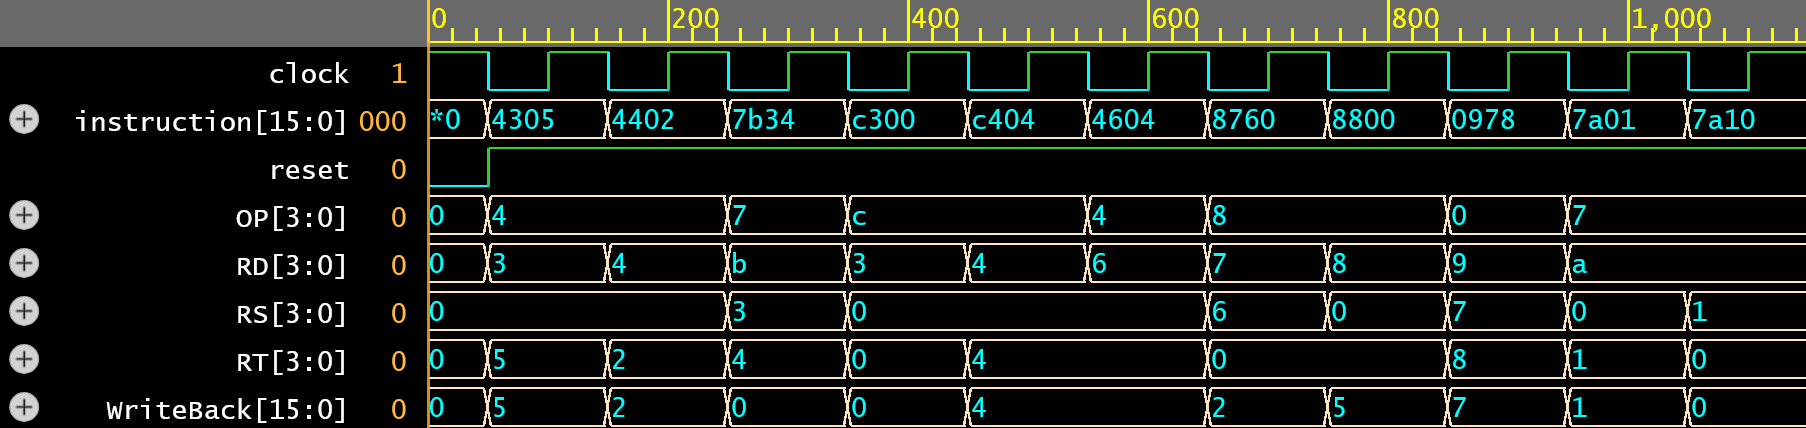
\includegraphics[width=0.95\textwidth]{CPU-waveform}
    \caption{The waveform for the CPU component.}
    \label{fig:CPU-waveform}
\end{figure}

\begin{table}[ht!]
    \centering
    \begin{tabular}{|l||c|c|c|c|c|} 
     \hline
     Instruction & op & rd & rs & rt & value (of rd) \\
     \hline
     \verb|ADDI R3,  R0,  5| & \verb|0x4| & \verb|0x3| & \verb|0x0| & \verb|0x5| & \verb|5| \\ 
     \hline                                                                             
     \verb|ADDI R4,  R0,  2| & \verb|0x4| & \verb|0x4| & \verb|0x0| & \verb|0x2| & \verb|2| \\
     \hline                                                                             
     %
     \verb|SLT  R11, R3, R4| & \verb|0x7| & \verb|0xB| & \verb|0x3| & \verb|0x4| & \verb|0| \\
     \hline                                                                             
     %
     \verb|SW   R3,   0(R0)| & \verb|0xC| & \verb|0x3| & \verb|0x0| & \verb|0x0| & \verb|0| \\
     \hline                                                                             
     \verb|SW   R4,   4(R0)| & \verb|0xC| & \verb|0x4| & \verb|0x0| & \verb|0x4| & \verb|4| \\ 
     \hline                                                                             
     %
     \verb|ADDI R6,  R0,  4| & \verb|0x4| & \verb|0x6| & \verb|0x0| & \verb|0x4| & \verb|4| \\
     \hline                                                                             
     %
     \verb|LW   R7,   0(R6)| & \verb|0x8| & \verb|0x7| & \verb|0x6| & \verb|0x0| & \verb|2| \\
     \hline                                                                             
     \verb|LW   R8,   0(R0)| & \verb|0x8| & \verb|0x8| & \verb|0x0| & \verb|0x0| & \verb|5| \\
     \hline
     %             
     \verb|ADD  R9,  R7, R8| & \verb|0x0| & \verb|0x9| & \verb|0x7| & \verb|0x8| & \verb|7| \\
     \hline                                                                             
     %
     \verb|SLT  R10, R0, R1| & \verb|0x7| & \verb|0xA| & \verb|0x0| & \verb|0x1| & \verb|1| \\
     \hline                                                                             
     \verb|SLT  R10, R1, R0| & \verb|0x7| & \verb|0xA| & \verb|0x1| & \verb|0x0| & \verb|0| \\
     \hline                                                                             
    \end{tabular}
    \caption{Results of the CPU component testbench in table form.}
    \label{table:CPU-waveform_table}
\end{table}


The CPU component works as expected. Figure \ref{fig:CPU-waveform} shows the waveform of the CPU
component, correctly outputting the results of each operation. The waveform is in hex radix to
easily show the instruction in the current clock cycle and the fact that the ALU does not have any
negative results. Table \ref{table:CPU-waveform_table} shows the waveform results in table form.

\section*{Conclusions}
The new \verb|slt| instruction was implemented into the CPU correctly, shown through the testbench
for the CPU. The knowledge from this lab was learning how to support the new \verb|slt| instruction
correctly. This was done by realizing that subtraction can be used for comparison by looking at the
difference's sign bit. Then, the control block component was adjusted to correctly supply the ALU
opcode, ensuring that the new instruction is seen as an R-type, and allowing the write back
multiplexer to support another connection.

% \newpage
% 
% \section*{References}
% \noindent
% [1]    Computer Organization 22104, EECS, University of Arkansas, “Lab 1,”  Sep. 17, 2024.
% 
% \noindent
% [2]    Computer Organization 22104, EECS, University of Arkansas, “Lab 2,”  Sep. 24, 2024.
% 
% \newpage
% 
% \section*{Appendix}
% \begin{figure}[h!]
%     \centering
%     \includegraphics[width=0.9\textwidth]{foo}
%     \caption{
%         Lorem ipsum dolor sit amet, qui minim labore adipisicing minim sint cillum sint consectetur
%         cupidatat.
%     }
%     \label{fig:foo}
% \end{figure}
% 
% \newpage
% 
% \begin{figure}[h!]
%     \centering
%     \includegraphics[height=0.4\textheight]{bar}
%     \caption{Lorem ipsum something something shorter sentence}
%     \label{fig:bar}
% \end{figure}
\end{document}
